%%
%% FrameSoC Workbench User Guide
%%

\documentclass[twoside]{article}
\usepackage[a4paper]{geometry}
\usepackage[utf8]{inputenc}
%\usepackage[T1]{fontenc}
\usepackage{RR}
\usepackage[hidelinks]{hyperref}
\usepackage{epsfig}
%\usepackage[english]{babel}
\usepackage{cite}
\usepackage{float}
\usepackage{graphicx}
\usepackage{subcaption}
\usepackage{textcomp}
\usepackage{wrapfig}

\usepackage{listings}
%%
%% date
\RRdate{June 2014}
%%
%%
\RRauthor{
Youenn Corre \thanks{INRIA, youenn.corre@inria.fr} \\
Damien Dosimont \thanks{INRIA, damien.dosimont@imag.fr} 
}

%% On each even page
\authorhead{Ocelotl User Guide}
%% French title
\RRtitle{Ocelotl User Guide}
%% English title
\RRetitle{Ocelotl User Guide}
%%
\titlehead{Ocelotl User Guide}
%%
\RRprojet{MOAIS}
%%
\URRhoneAlpes 
%%
\RCGrenoble 
%%
\abstract{This guide describes the Ocelotl tool, delivered within the SETv1.0 of the FrameSoC framework.}

%%=====================================================================
%%=====================================================================
\begin{document}

\begin{sloppypar} %% avoid long words exceeding margins
%%=====================================================================
%%=====================================================================

%\shorthandoff{:} %% Remove the space before the colon
\interfootnotelinepenalty=10000 %% allow long footnotes

%%=====================================================================
%% Custom commands
\newcommand{\parag}[1]{\paragraph{#1}\mbox{}\\}
\newcommand{\subparag}[1]{\subparagraph{#1}\mbox{}\\}
\newcommand{\subsubparag}[1]{\subparagraph{#1}}
%% 
%% Itemize
\renewcommand{\labelitemi}{$\bullet$}
\renewcommand{\labelitemii}{$\circ$}
%%=====================================================================

%%
\makeRT 
%%

%%=====================================================================
\renewcommand{\contentsname}{Table of contents}
\tableofcontents
\newpage
%%=====================================================================
%=====================================================================
\section{Introduction}
\label{intro}

%=====================================================================

Ocelotl is a tool to explore, analyze and visualize execution traces through aggregation techniques. It is part of the SoC-Trace project, and as such, it is integrated in the FrameSoC framework as an Eclipse plugin. 

%\section{Installation}
%Ocelotl come as an Eclipse plugin installed with the 


\section{Launching Ocelotl}

\begin{figure}[h!]
	\centering
    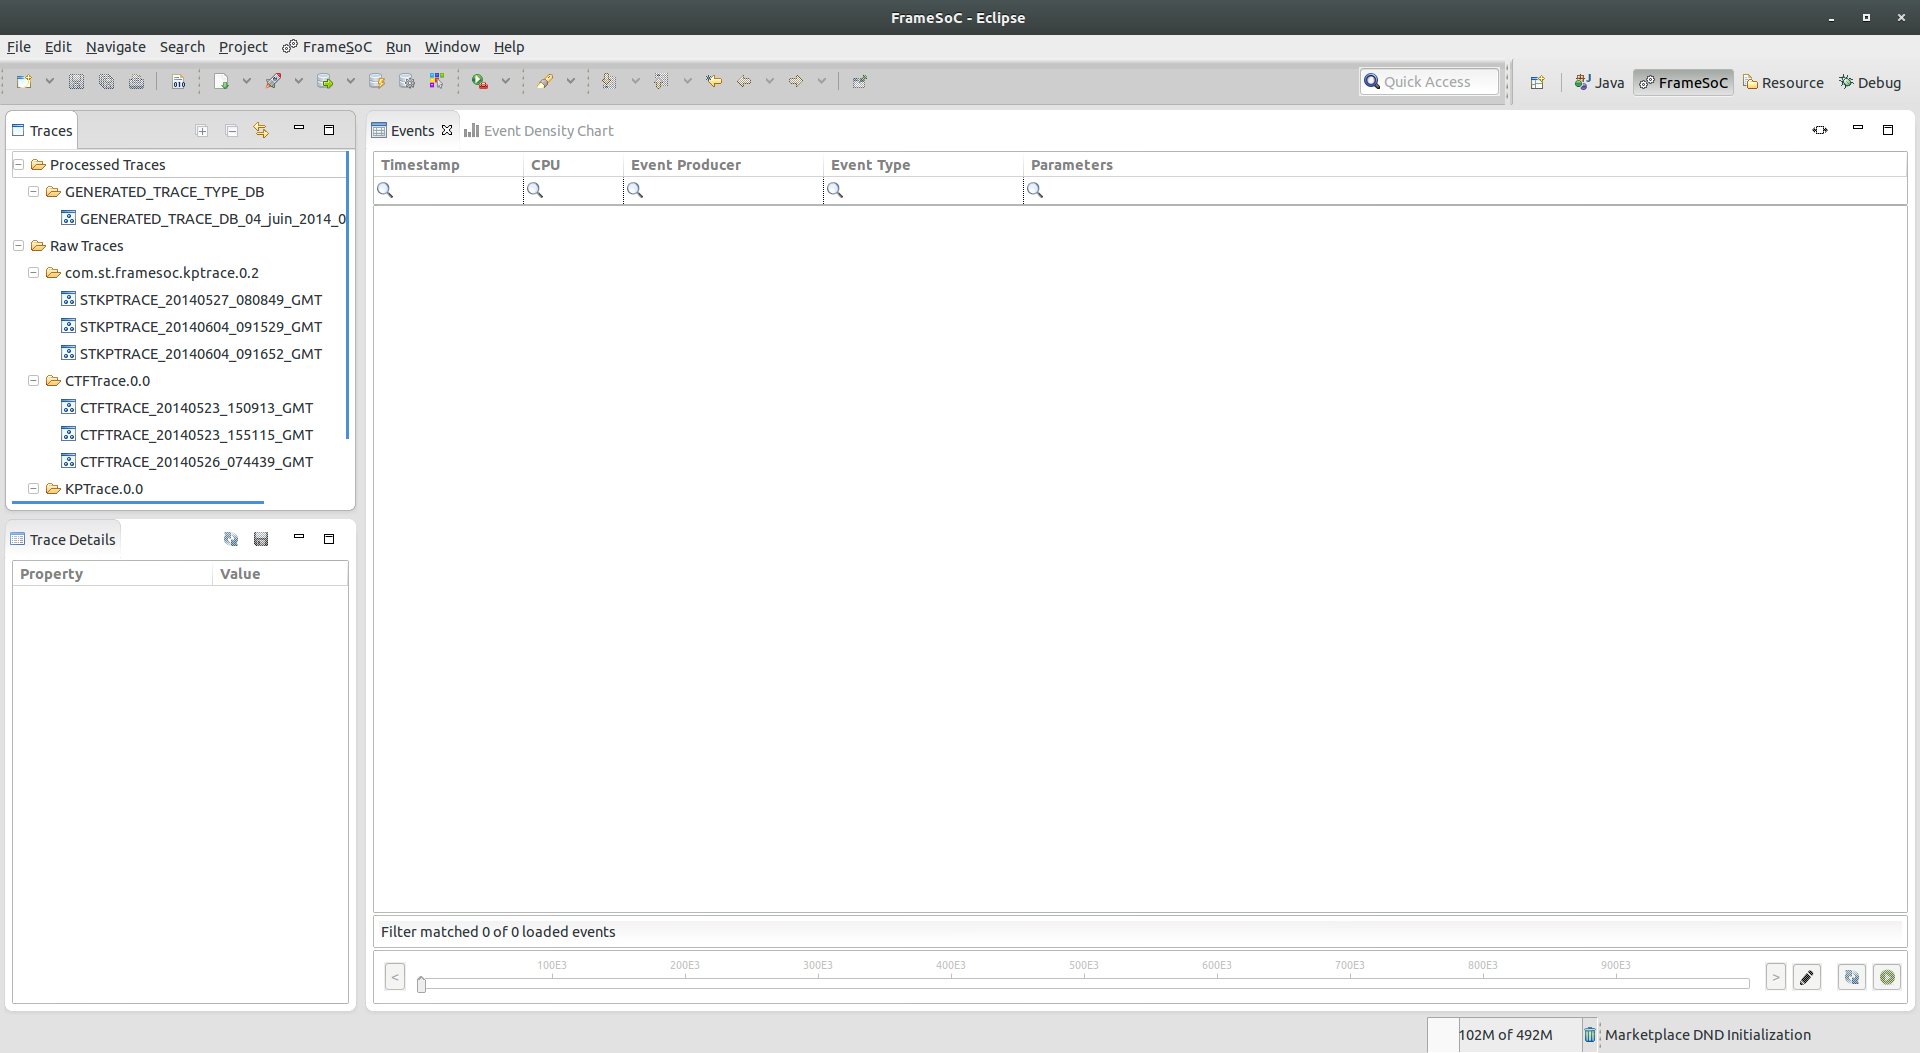
\includegraphics[width=1.0\textwidth]{images/framesoc_launch.png}
	\caption{FrameSoC Eclipse Workbench at startup}
	\label{frameLaunch}
\end{figure}

In order to launch Ocelotl:
%begin{wrapfigure}{R}{0.5\textwidth}
% 		\begin{center}
%   			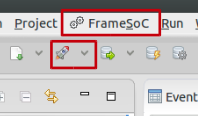
\includegraphics[width=0.38\textwidth]{images/labeled.png}
%  		\end{center}
%  		\caption{The FrameSoC menu and the \textit{Analyse Trace} icon}
%	\end{wrapfigure}
\begin{enumerate}
	\item 
	\begin{itemize}
		\item Go to the FrameSoC menu, choose the \textit{Trace Analysis} entry and click on \textit{Launch Analysis Tool}. 
		\item Or click on the \textit{Analyse Trace} icon.
	\end{itemize}

	\begin{figure}[h!]
		\centering
		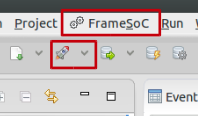
\includegraphics[scale=0.5]{images/labeled.png}
		\caption{The FrameSoC menu and the \textit{Analyse Trace} icon}
		\label{launchOcelotl}
	\end{figure}
	
	\item Select the Ocelotl tool.
	\begin{figure}[h!]
		\centering
		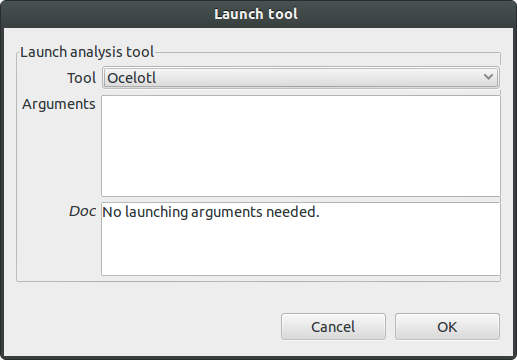
\includegraphics[scale=0.5]{images/launch_tool.png}
		\caption{Ocelotl launching window}
	\end{figure}
	\item No argument is needed so just click \textit{OK}.
\end{enumerate}

The Ocelotl tool view should open, as illustrated in Fig. \ref{ocelotlOverview}.
\begin{figure}[h!]
	\centering
	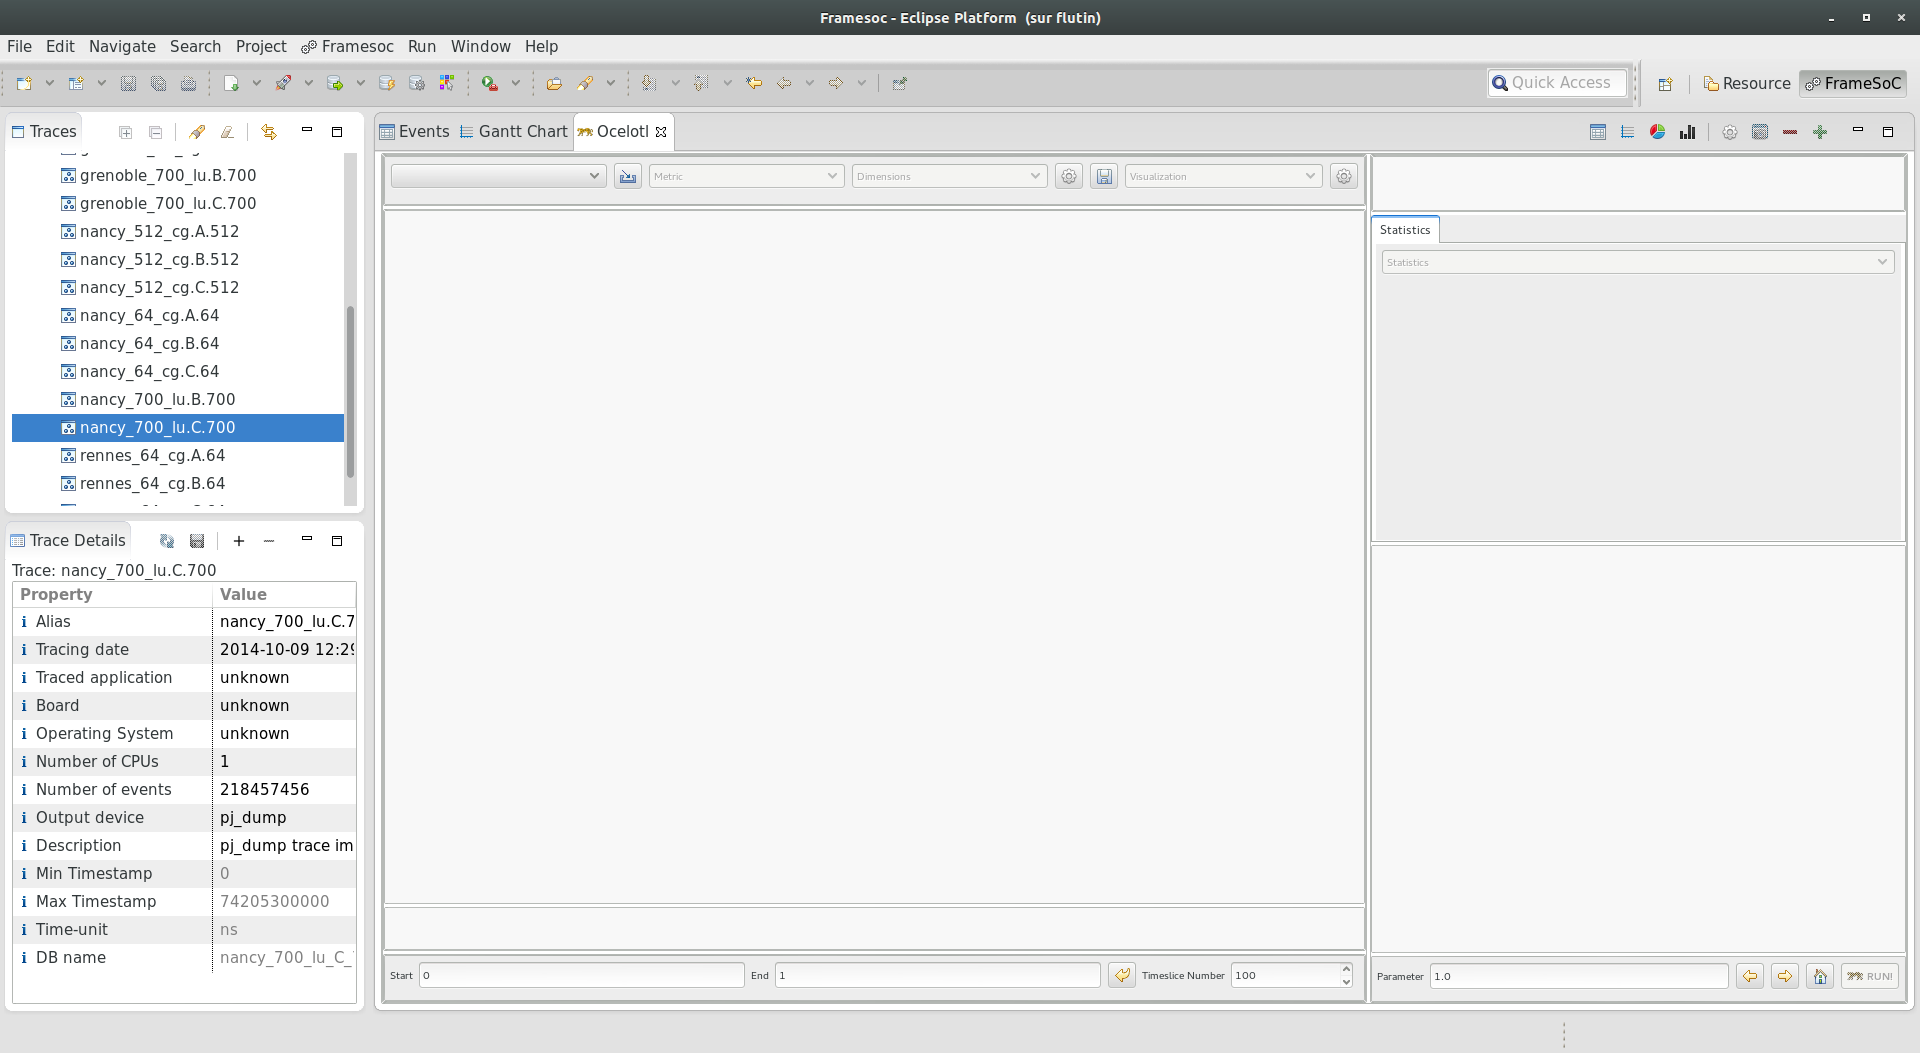
\includegraphics[width=1.0\textwidth]{images/ocelotl_startup.png}
	\caption{Ocelotl at startup}
	\label{ocelotlOverview}
\end{figure}


\section{Ocelotl Features}
In this section, we describe how to load a trace, launch the analysis and explore the results by modifying parameters. 

\subsection{Loading a trace}
\begin{figure}[h!]
	\centering
	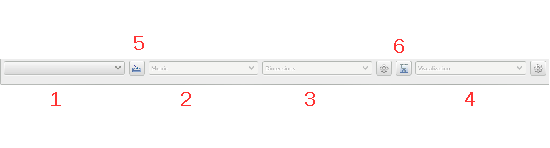
\includegraphics[scale=0.7]{images/traceSelection_labeled.pdf}
	\caption{Trace configuration interface}
	\label{traceConf}
\end{figure}

\subsubsection{Select a trace}

In the top right corner of Ocelotl, the \textit{Trace Overview} tab allows to select a trace to analyze (element \textcolor{red}{1} in Fig. \ref{traceConf}).

\subsubsection{Microscopic Description Settings}
Once a trace is selected, the \textit{Microscopic Description} combo becomes available (element \textcolor{red}{2} in Fig. \ref{traceConf}). It displays the operators compatible with the current trace. At the moment, the available operators are: 
\begin{itemize}
	\item The \textit{Event Distribution}, that performs an analysis based on the event occurrences. This type of analysis is compatible with all the traces.
	\item The \textit{State Distribution}, that performs an analysis based on the event duration. This analysis requires the trace to contains events of the type state.
	\item The \textit{Variable Distribution}, that performs an analysis based on the variation of the value of the event over time. This analysis requires the trace to contains events of the type variable.
\end{itemize}

Once the type of distribution selected, you can configure the analysis by clicking on the \textit{Settings} button, which opens a setting window (cf. Figure \ref{microSettings}). 
\begin{figure}[h!]
	\centering
	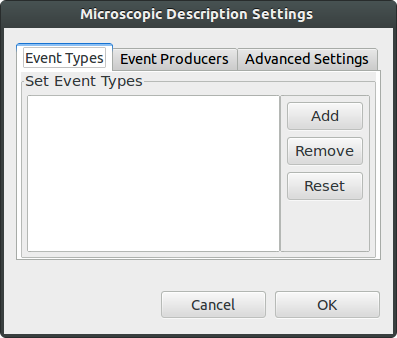
\includegraphics[scale=0.6]{images/state_settings.png}
	\caption{Microscopic Description Settings}
	\label{microSettings}
\end{figure}
By default, all the event types and all the event producers are selected. The available settings are:

\begin{itemize}
	\item in the \textit{Event Types} tab, you can filter the event types involved in the analysis;
	\item in the \textit{Event Producers} tab, you can filter the event producers (the resources that produce the events) involved in the analysis. The \textit{Add Result} button enables to load a set of event producers saved as an analysis result by another tool;
    \item in the \textit{Advanced Settings} tab, you can configure some advanced settings\footnote{\textbf{Note:} Modifying these values might decrease the trace reading performances.}:
	\begin{itemize}
		\item \textit{Event Number Retrieved by Threads}: set how much events are loaded by threads for each iteration during the trace reading.
        \item \textit{Event Producers per Query}: enables to divide the query into several queries with a fixed number of event producers. This functionality is useful if the disk space is low, as the temp directory is used to store the query result during the trace reading. The default value is 0 which corresponds to fetching all producers in one query.
        \item \textit{Working Threads}: set the number of active threads during the trace reading. 
	\end{itemize}
\end{itemize}

\subsubsection{Visualization Settings}
Once a distribution is selected, the \textit{Visualization} combo (element \textcolor{red}{3} in Fig. \ref{traceConf}) automatically selects the \textit{Proportions} view, if available, otherwise you have to choose one manually. The currently available choices are:
\begin{itemize}
	\item \textit{Parts}: for a visualization showing aggregates that correspond to an homogeneous behavior in the trace. The aggregates are separated by a blank space and all have a different color. In \textit{Settings}, the available parameters are:
	\begin{itemize}
		\item \textit{Aggregate parts}: gathers time slices that belong to the same aggregate. If not active, each time slice is separated, and their aggregation is shown thanks to their color.
		\item \textit{Show part number}: attributes a number to each aggregate to help distinguishing them.
	\end{itemize}
		\item \textit{Proportions}: for a visualization showing the same aggregates as in \textit{Parts}, but also the proportion of event occurrences (or the ratio of state duration, if state distribution was selected in the previous step) for each aggregate. In this visualization, each event/state is separated vertically in each aggregate and their proportion is shown by making the height of each event/state in an aggregate proportional to its occurrence/duration. The events/states that have a proportion too small to be visible, are aggregated and displayed on top of the aggregate as a dotted line. In the \textit{Settings} window, you can customize the color of each event.
\end{itemize}

\subsection{Quality Curves}
Ocelotl displays curves representing the different aggregation levels, as shown in Fig. \ref{aggregCurves}. %The X axis is the aggregation ratio from 1 to 0. %(pIC), and the Y axis is the %TODO what is it ?
The green curve is the complexity and the red is the information.

\begin{figure}[h!]
	\centering
	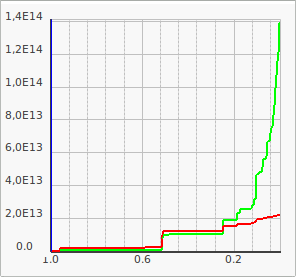
\includegraphics[scale=0.5]{images/ocelotlCurves.png}
	\caption{Quality curves in rising order.}
	\label{aggregCurves}
\end{figure}
The tab \textit{Quality Curves} enables to change the appearance of complexity and information curves provided by the aggregation algorithm:
\begin{itemize}
	\item \textit{Normalize Qualities}: normalizes the curves and scale them on the interval [0:1], which improves their readabilty.
    \item You can choose between two representations of the curves: rising curves (complexity gain, information gain) or decreasing curves (complexity reduction, information loss).
    \item The \textit{Threshold} parameter determines the quality curves precision. The more its value decreases, the more the precision increases and the more aggregation steps are found. However, setting a too small value may lead to bad performances, so we advice to keep the default value.
\end{itemize}

%\subsubsection{Threshold}


\subsection{Time settings}
In order to tune the time settings, several parameters can be modified in the bar under the graph display area (Figure \ref{timeSettings}).
 
\begin{figure}[h!]
	\centering
	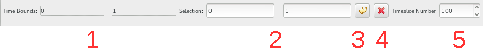
\includegraphics[width=1.0\textwidth]{images/ocelotl_bottom_time.pdf}
	\caption{Time Settings}
	\label{timeSettings}
\end{figure}

\subsubsection{Time Stamps}
You can change the trace time bounds thanks to the \textit{Start} and \textit{End} fields (\textcolor{red}{1} and \textcolor{red}{2} resp. in Figure \ref{timeSettings}) at the bottom of the window. By default, after loading a trace, the values are the starting and ending timestamps of the trace. If an area of the graph is selected, or if a zooming operation is performed, the displayed values are the starting and ending timestamps of the selected area. The \textit{Reset} (\textcolor{red}{3}) button enables to get the original values back.

\subsubsection{Time Slices}
The \textit{Timeslice Number} field (\textcolor{red}{4}) corresponds to the number of time slices that will be used to compute the aggregation. It is advised to tune this parameter in order to find a granularity that is convenient to the analysis. As the aggregation algorithm complexity is dependent on this parameter, it is advised to increment it progressively to keep good performances.

\subsection{Analysis settings}
To analyze the trace, several parameters allows to explore  different levels of aggregation and view. The aggregation settings are located under the \textit{Quality curves} display.
 
\begin{figure}[h!]
	\centering
	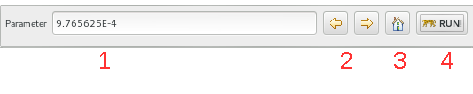
\includegraphics[scale=0.8]{images/aggregationSettings.pdf}
	\caption{Aggregation Settings}
	\label{aggregSettings}
\end{figure}

\subsubsection{Run an Analysis}
After having set the configuration, click on RUN! (\textcolor{red}{3} in Fig. \ref{aggregSettings}) (or press ENTER on the keyboard). The aggregation is then computed. This operation can take a while. When it is finished, the visualization and the curves are shown, as illustrated in Fig. \ref{showAggreg}.


\subsubsection{Change the Aggregation strength}
In order to find a relevant aggregation, you can tune the \textit{Parameter} setting. This parameter allows to explore different aggregation levels, by navigating between different balances of the information loss and the gain in complexity. There are three ways to do this:
\begin{enumerate}
	\item Click on the curves. The corresponding parameter value is retrieved, and used to show the associated aggregation.
	\item Use the $<$ and $>$ buttons (\textcolor{red}{2}) (or use left and right arrows on the keyboard). It enables to increment or decrement the parameter.
	\item Enter a value manually, in the \textit{Parameter} field (\textcolor{red}{1}). The value must be between 1 and 0.
\end{enumerate}
A value of 1 means that the aggregation strength is maximal: all the trace is disaggregated. On the opposite, a value of 0 means that each time slice is disaggregated. An intermediate value provides a compromise between both extrema.

\subsubsection{Zoom}
Once you obtain an interesting aggregation level, you may want to focus on a particular time area. You can zoom in on the trace by selecting an area by clicking and dragging with the left button of the mouse. Then, click on RUN! or press ENTER to display the selected area. In order to zoom out, you must click on \textit{Reset} and then on RUN!, to show the global view of the trace.

\subsubsection{Switch to an Event table}
%If a generic Gantt Chart is available, 
You can display the trace in an event table by clicking on the corresponding button in the top right corner. The table will show the events of the trace that are within the time bounds shown in the \textit{Start} and \textit{End} fields. You can focus on an area by selecting it with the mouse left button drag and then switching directly to the event table, without loading the aggregation with the RUN! button. In future releases, it will also be possible to switch to a Gantt Chart (not available in SET 1.0).


\subsection{Graph Display}
\begin{figure}[h!]
	\centering
	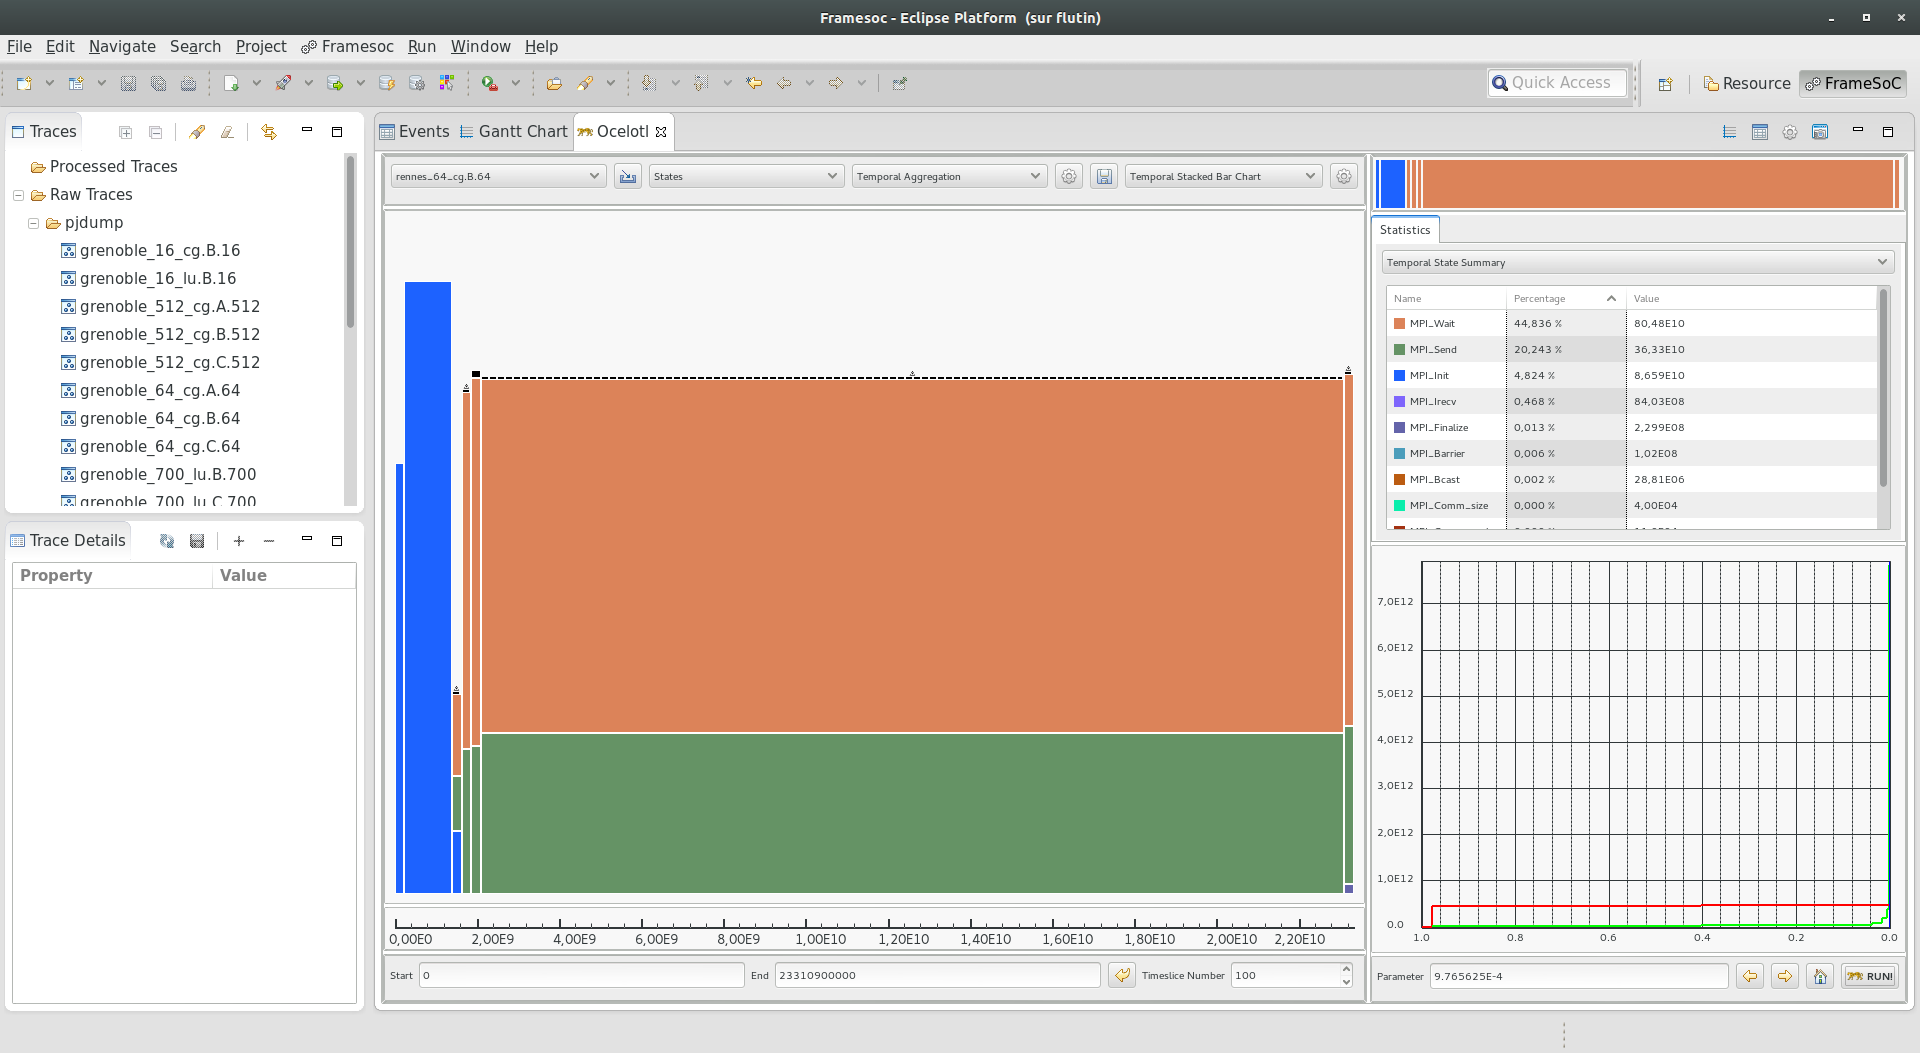
\includegraphics[width=1.0\textwidth]{images/ocelotl_aggregated.png}
	\caption{A graph showing an aggregated trace}
	\label{showAggreg}
\end{figure}

Figure \ref{showAggreg} shows an aggregated trace, with the proportion view. At the bottom of the graph, a time axis shows the time stamps of the currently displayed events. Events of different types have different colors. By letting the mouse over a part of the graph for a short time, a tooltip note shows the type of events represented by that part of the graph. For the event view, this note also displays the number of occurrences of the events divided by the duration of the aggregate\footnote{The time unit of the trace is displayed in the \textit{Trace Details} tab on the left bottom of the screen.}. For the state view, it is the state duration divided by the aggregate duration.

\subsection{Known Issues}
You may need to redimension manually the different views, according to your resolution.

\newpage

%% bibliography
\newpage
\bibliographystyle{unsrt}
\bibliography{ocelotl_biblio}{}
%%

%%=====================================================================
%%=====================================================================
\end{sloppypar} 
\end{document}
%%=====================================================================
%%=====================================================================

\endinput
%%
%% End of file.
